\documentclass[hidelinks,12pt]{article}
\usepackage[utf8]{inputenc}
\usepackage[table,xcdraw]{xcolor}
\usepackage{mathtools}
\usepackage{amsthm}
\usepackage{amsmath}
\usepackage{amsfonts}
\usepackage{amssymb}
\usepackage{centernot}
\usepackage{marvosym}
\usepackage{enumitem}
\usepackage{hyperref}
\setcounter{tocdepth}{1}
\let\marvosymLightning\Lightning
\newtheorem{theorem}{Theorem}
\newtheorem{corollary}{Corollary}[theorem]
\newtheorem*{remark}{Remark}
\renewcommand\qedsymbol{QED}
\newcommand{\C}{\mathbb{C}}
\newcommand{\R}{\mathbb{R}}
\newcommand{\N}{\mathbb{N}}
\newcommand{\Z}{\mathbb{Z}}
\newcommand{\Q}{\mathbb{Q}}
\newcommand{\divby}{%
  \mathrel{\text{\vbox{\baselineskip.65ex\lineskiplimit0pt\hbox{.}\hbox{.}\hbox{.}}}}%
  }
\newcommand{\notdivby}{\centernot\divby}
\title{\scalebox{2}{Math 531 Homework 6}}
\author{\scalebox{1.5}{Theo Koss}}
\date{March 2021}
\begin{document}
\graphicspath{{/home/theo/Documents/GitHub/Math-Homeworks/Math 531/Random/}}
\maketitle
\section{Section 3.5}
\begin{itemize}
\item Problem 3: Give the subgroup diagrams of the following groups.\begin{enumerate}[label=(\alph*)]
    \item $\Z_{24}$\newline\scalebox{.1}{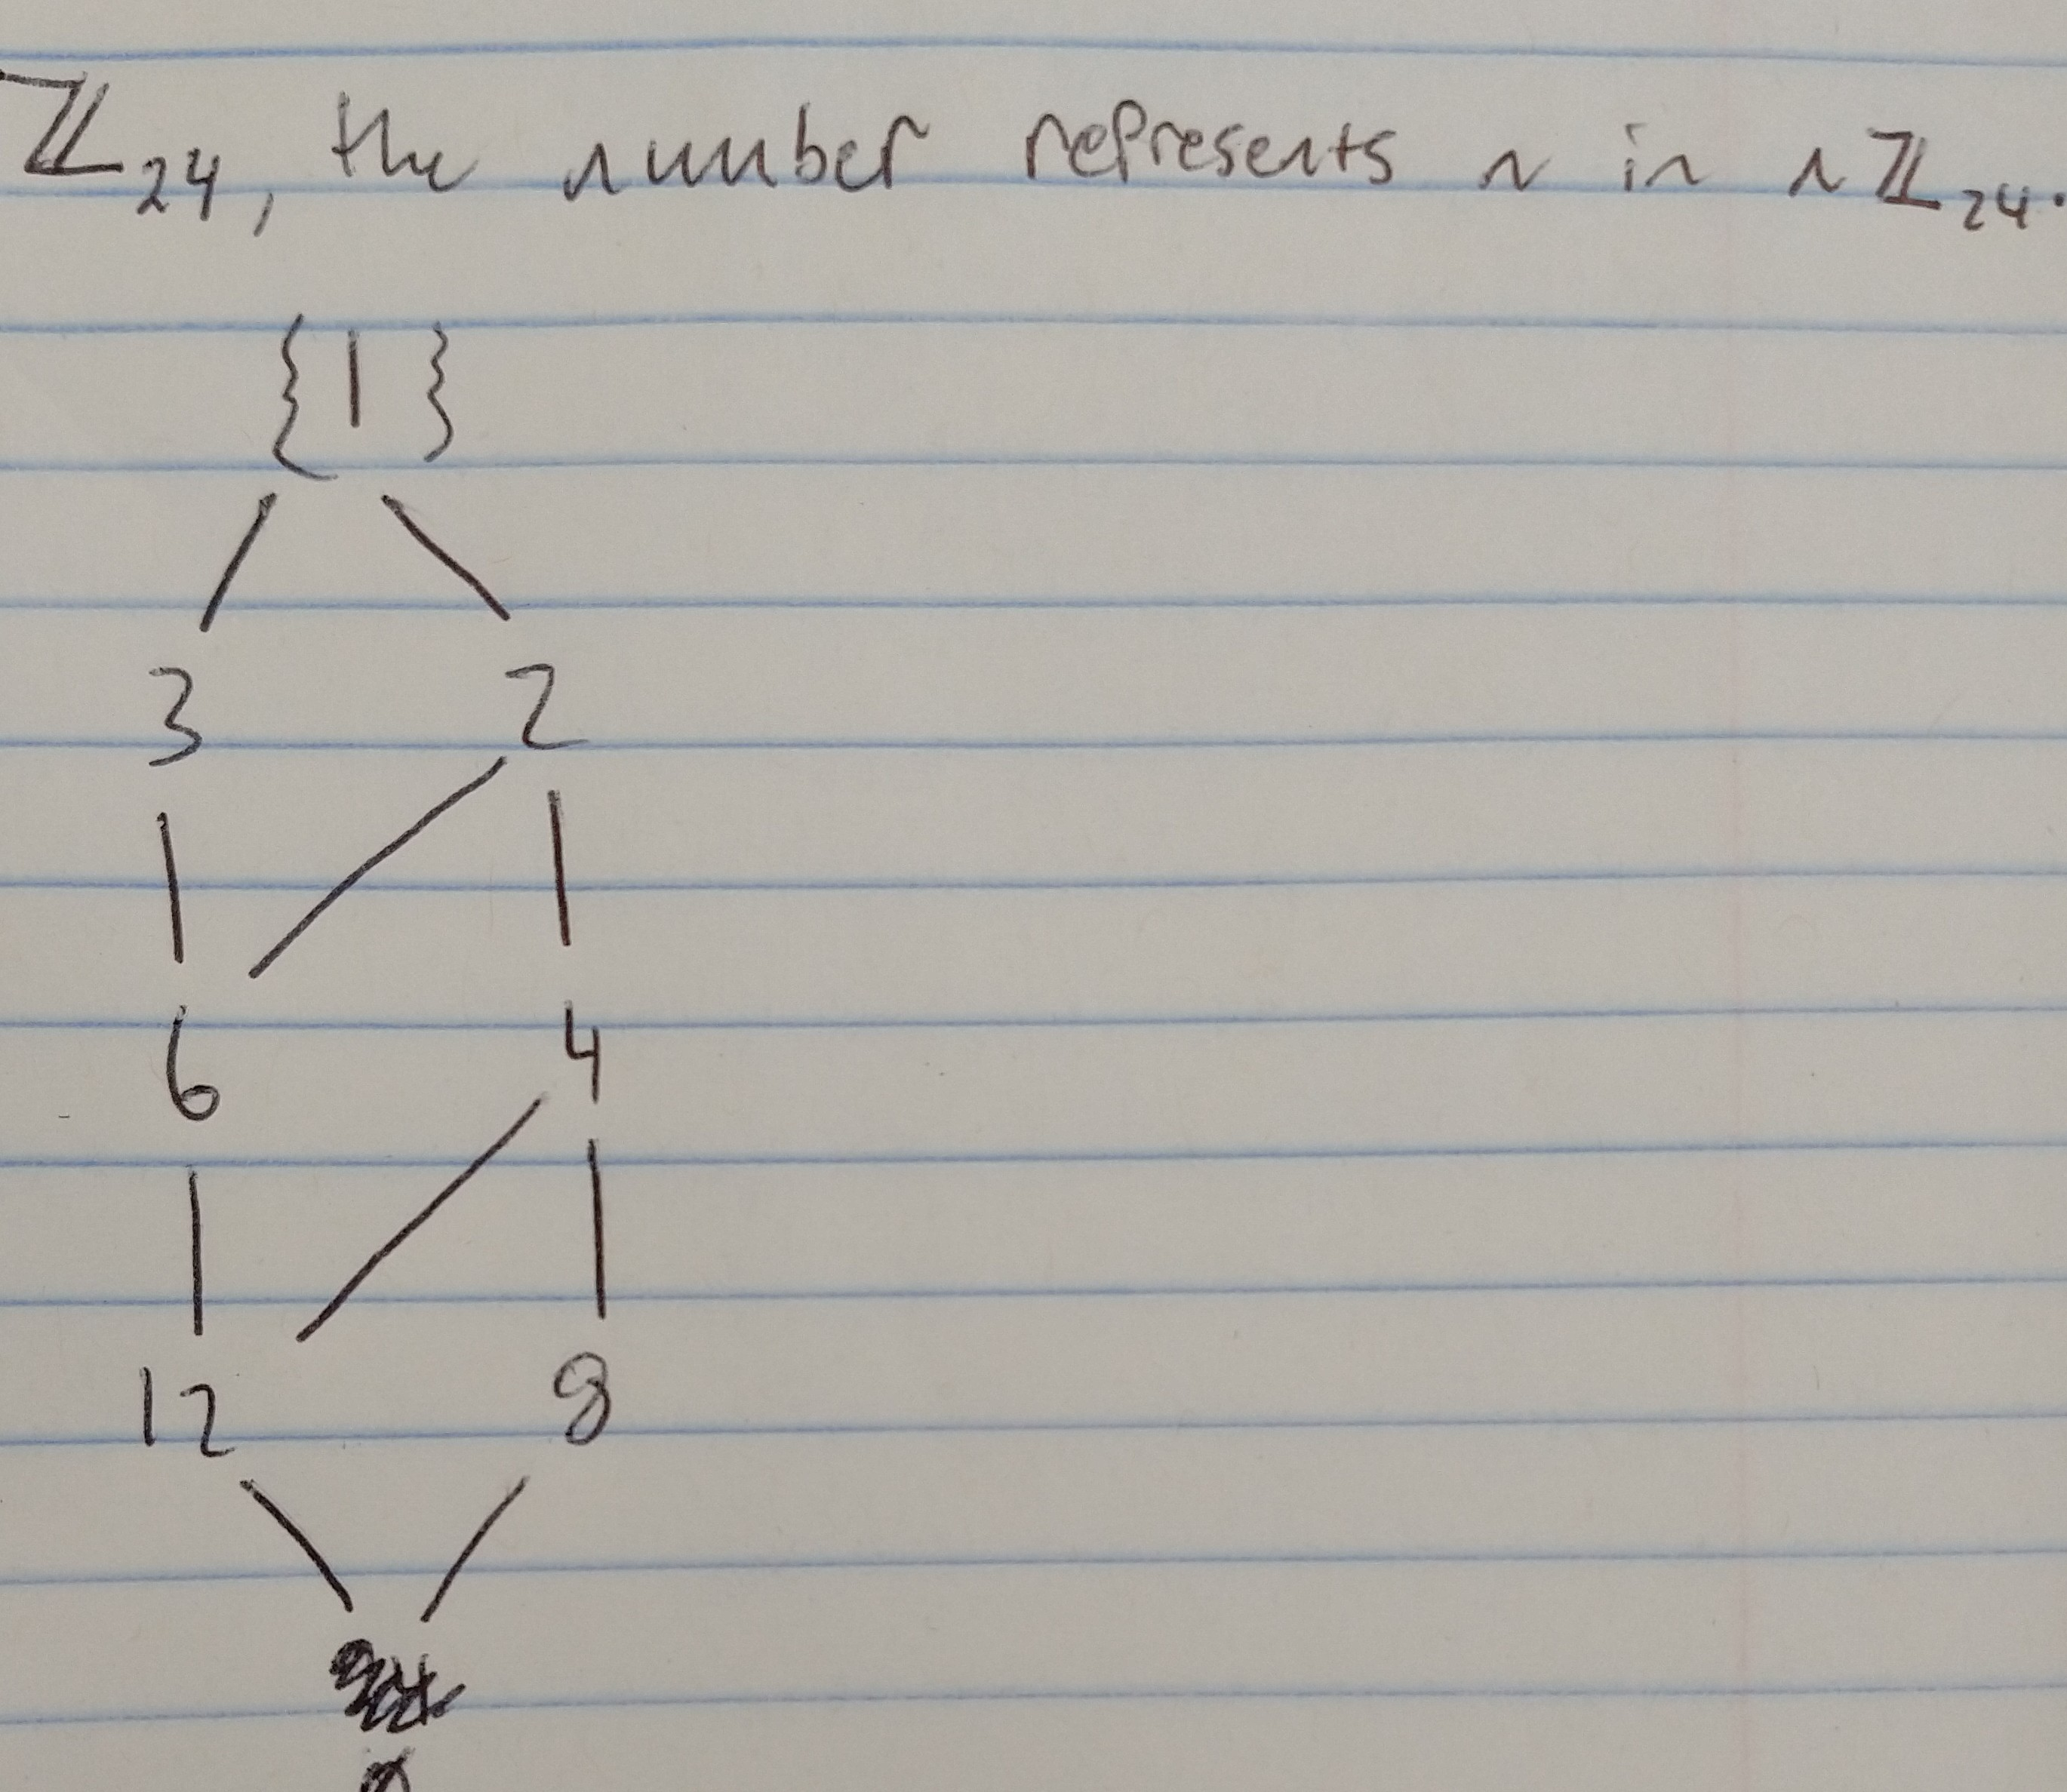
\includegraphics{z24.jpg}}
    \item $\Z_{36}$\newline\scalebox{.1}{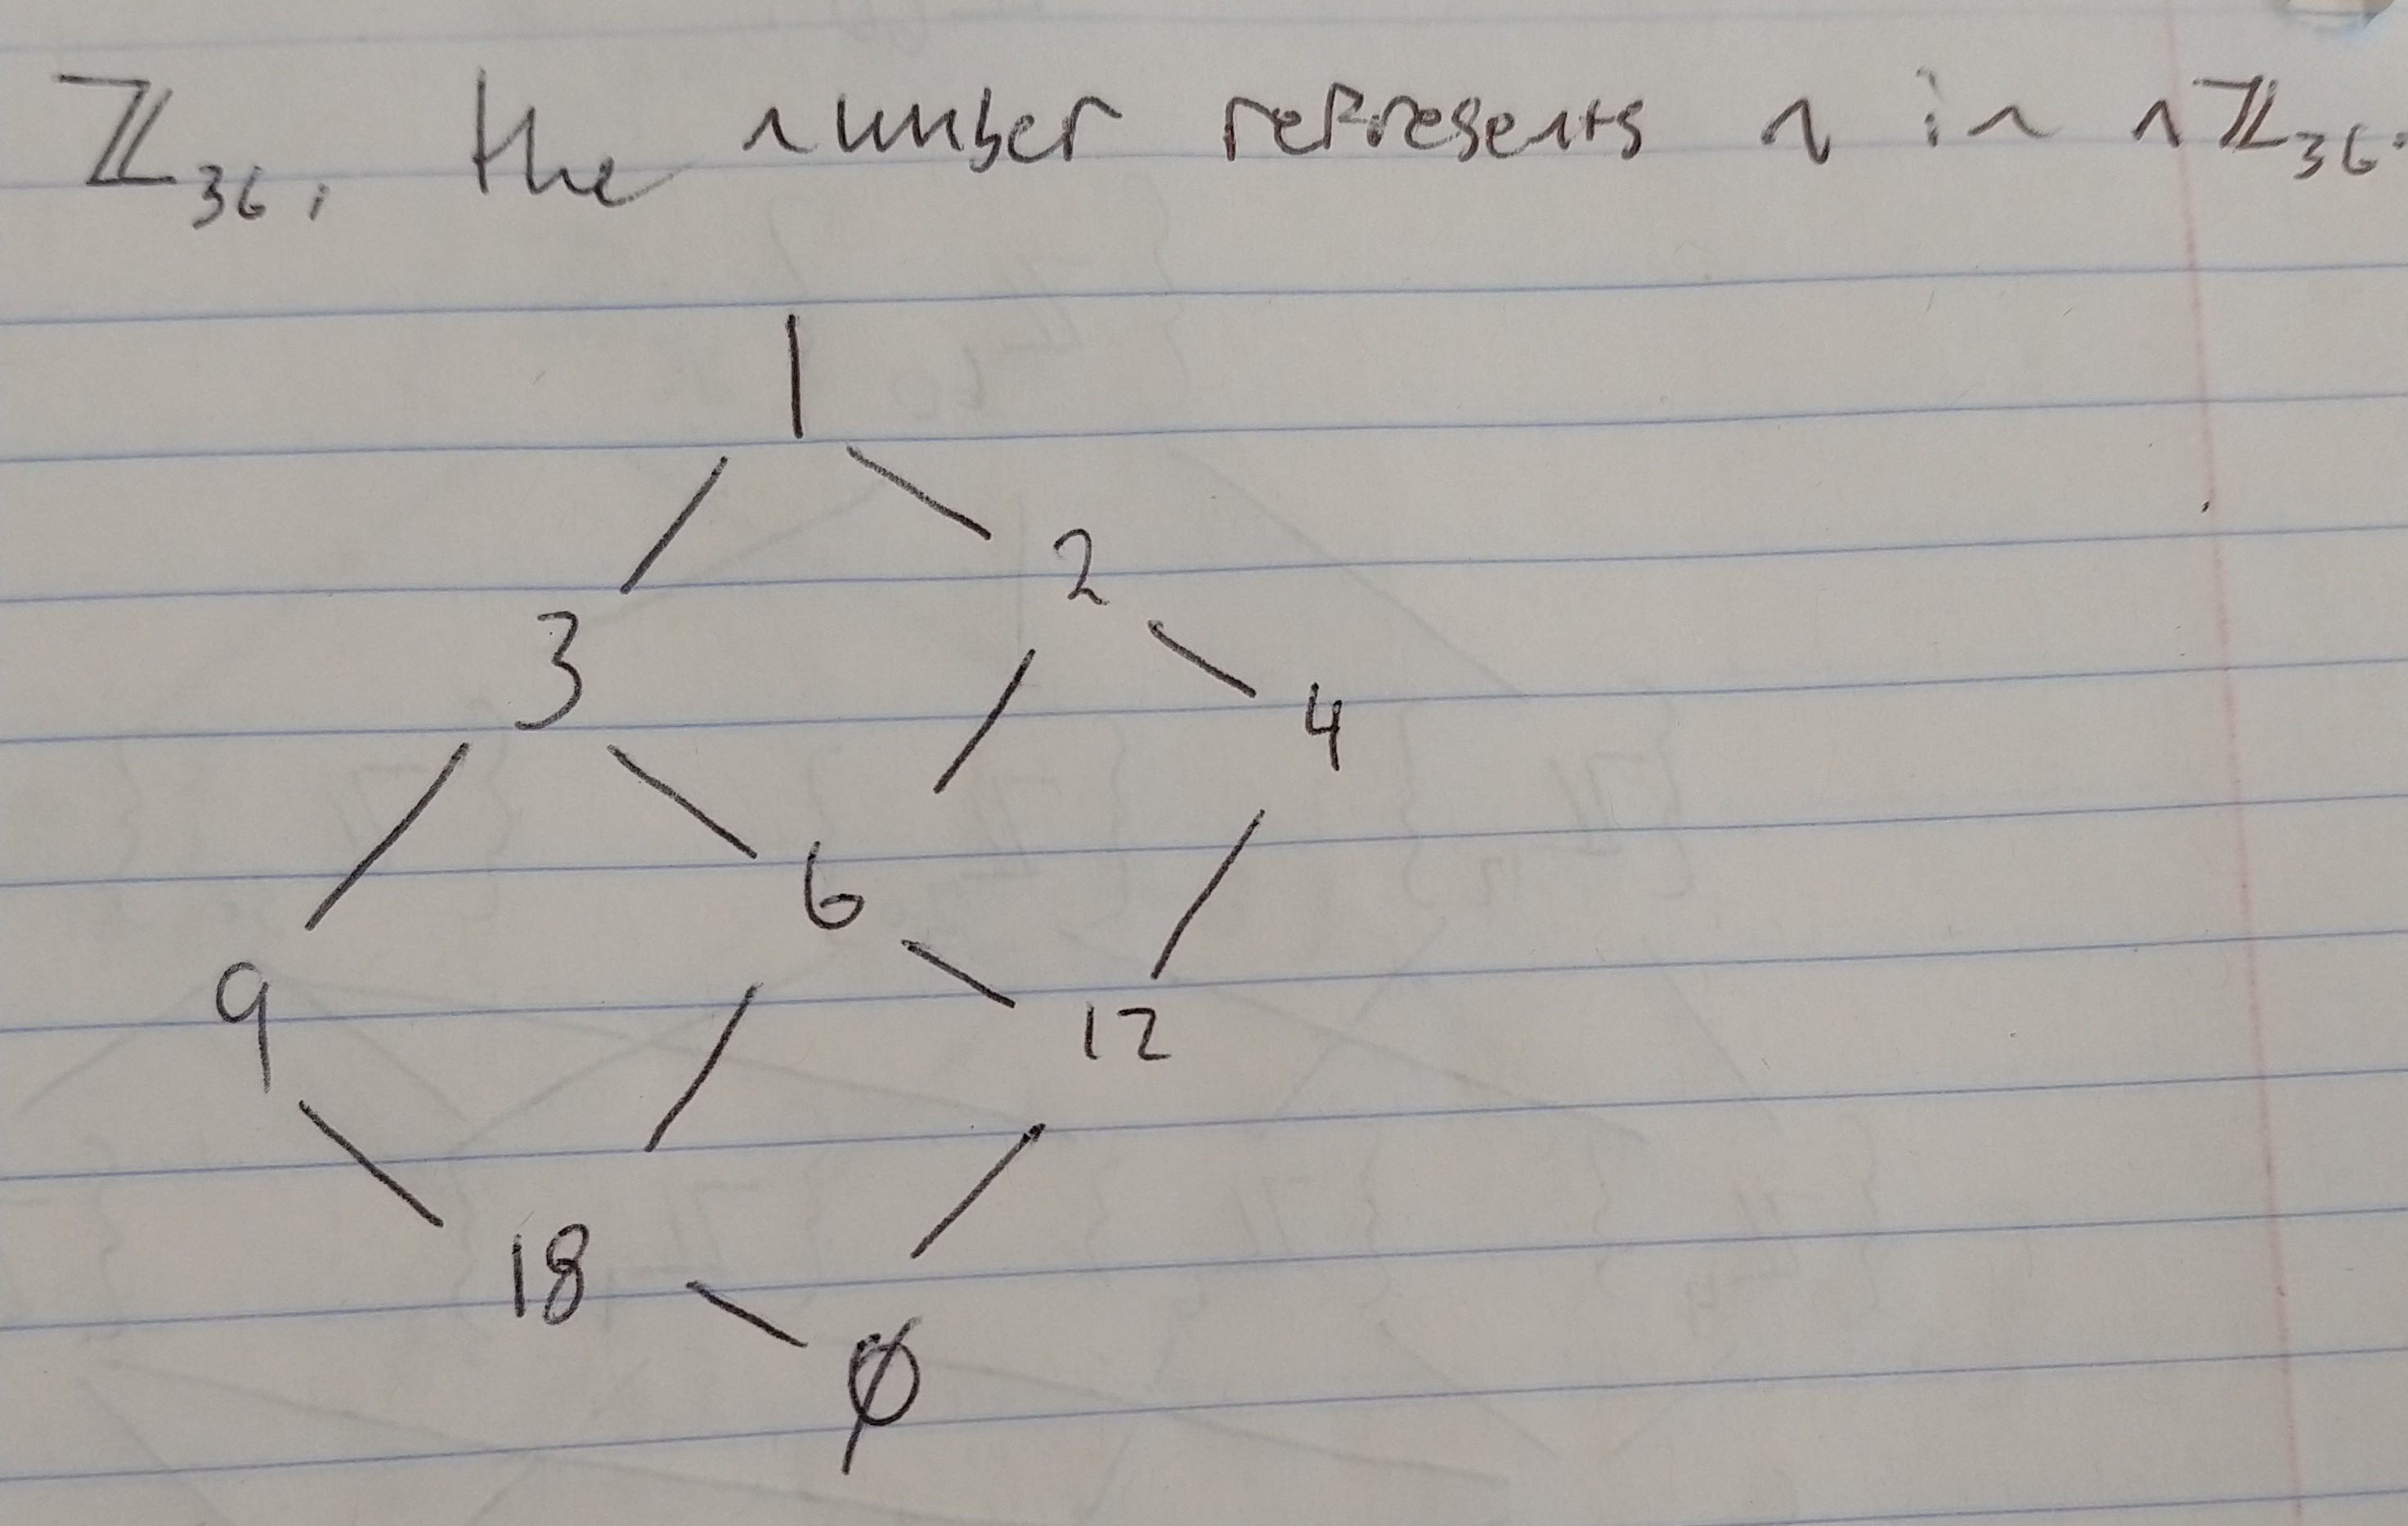
\includegraphics{z36.jpg}}
\end{enumerate}
\item Problem 4: Give the subgroup diagram of $\Z_{60}$.\newline\scalebox{.1}{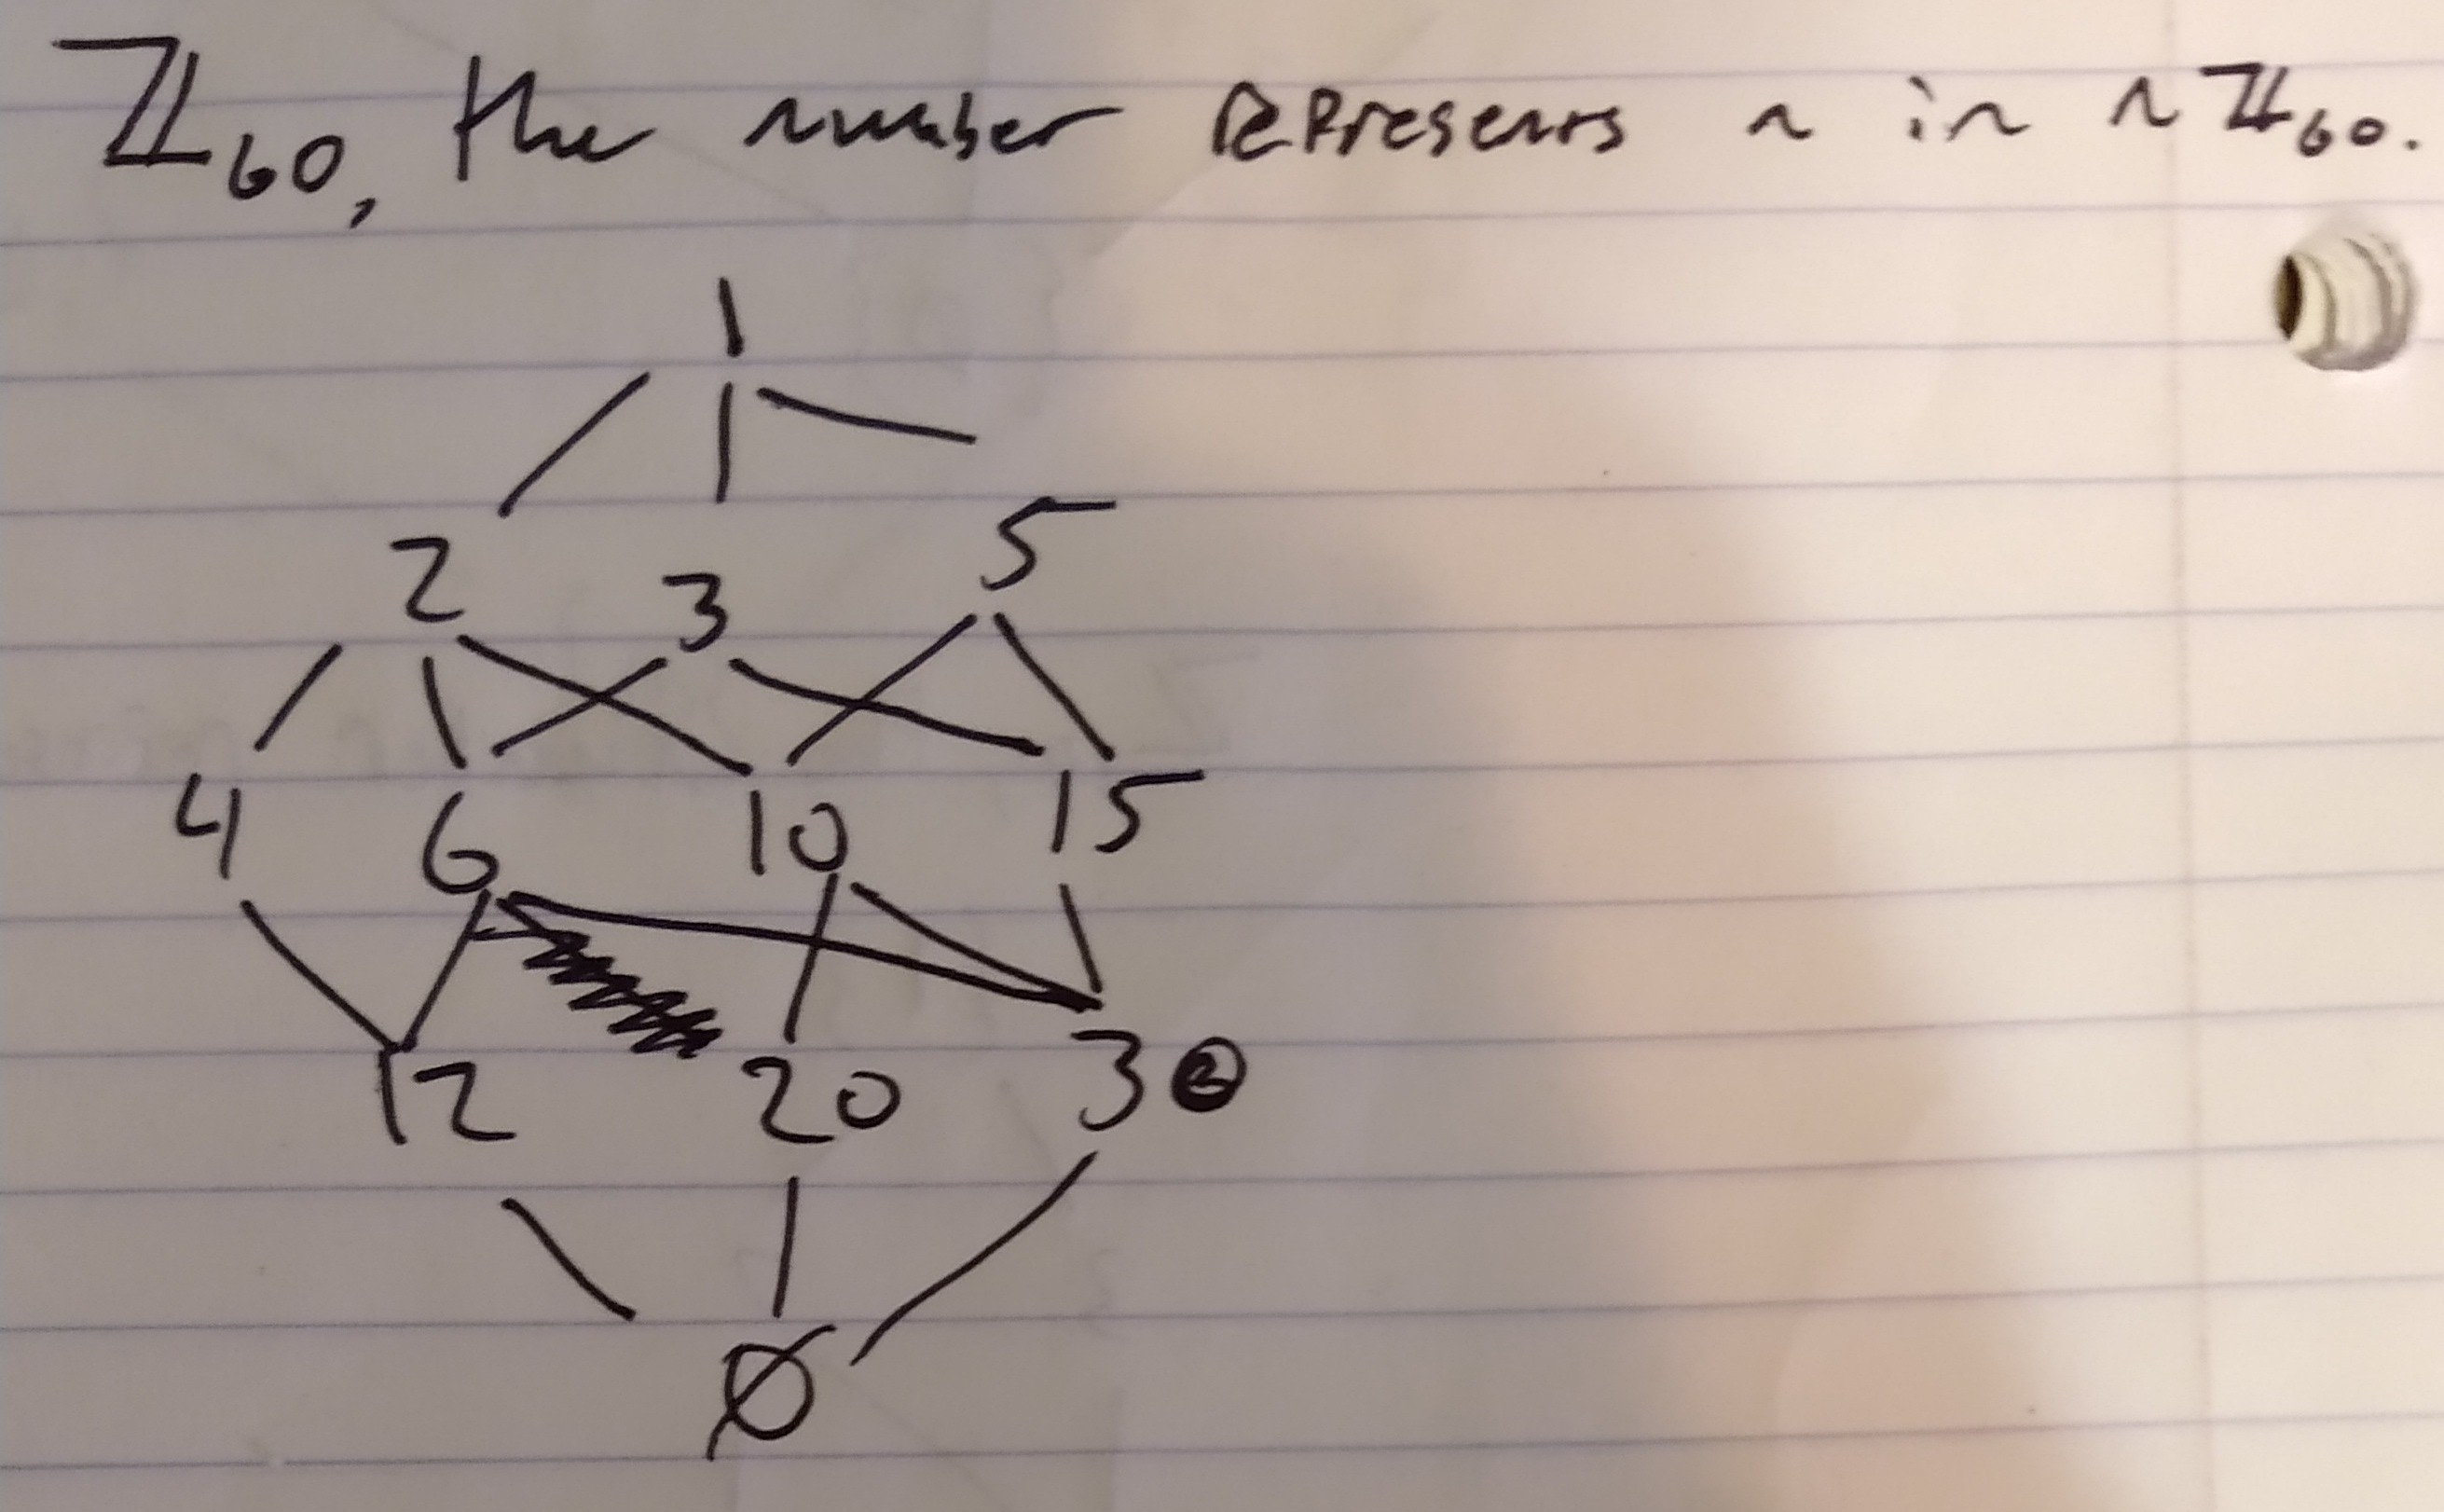
\includegraphics{z60.jpg}}
\item Problem 11: Which of the multiplicative groups, $\Z^{\times}_7$, $\Z^{\times}_{10}$, $\Z^{\times}_{12}$, $\Z^{\times}_{14}$ are isomorphic?\newline \begin{remark}Two finite cyclic groups of the same order are isomorphic. \href{https://proofwiki.org/wiki/Cyclic_Groups_of_Same_Order_are_Isomorphic}{\color{cyan}Proof.} \end{remark}\begin{enumerate}
    \item $\Z^{\times}_7$ is cyclic with generator 3, $|(\Z^{\times}_7)|=6$.
    \item $\Z^{\times}_{10}$ is cyclic with generator 3. $|\Z^{\times}_{10}|=9$.
    \item $\Z^{\times}_{12}$ is isomorphic to the klein 4-group, which is noncyclic. $|\Z^{\times}_{12}|=4$.
    \item $\Z^{\times}_{14}$ is cyclic with generator 3. $|\Z^{\times}_{14}|=6$.
\end{enumerate}Therefore, by our remark, $\Z^{\times}_{14}\cong\Z^{\times}_7$, since they are both cyclic groups of the same order.
\item Problem 21: Prove that if $p$ and $q$ are different odd primes, then $\Z^{\times}_{pq}$ is not a cyclic group.\begin{proof} By the Chinese Remainder Theorem, since $\gcd(p,q)=1$, it follows that $\Z^{\times}_{pq}$ is isomorphic to $\Z^{\times}_p\times\Z^{\times}_q$. Of course, $\Z^{\times}_p$ $\Z^{\times}_q$ are finite abelian groups, of order $p-1$ and $q-1$, respectively. And since $p,q$ are odd primes, $p-1$ and $q-1$ are both divisible by 2, therefore they are not coprime. By the Fundamental Theorem of Finitely Generated Abelian Groups, the product of two finite abelian groups of non-coprime orders is never cyclic. 
\end{proof}
\end{itemize}
\section{Section 3.6}
\begin{itemize}
\item Problem 1: Find the orders of each of these permutations.\begin{enumerate}[label=(\alph*)]
    \item $(1,2)(2,3)(3,4)=(1,2,3,4)$, order 4.
    \item $(1,2,5)(2,3,4)(5,6)=(1,2,3,4,5,6)$ order 6.
    \item $(1,3)(2,6)(1,4,5)=(1,4,5,3)(2,6)$ order $lcm(4,2)=4$.
    \item $(1,2,3)(2,4,3,5)(1,3,2)=(1,5,3,4)(2)$ order $lcm(4,1)=4$.
\end{enumerate}
\item Problem 3: Write out the addition table for $\Z_4\times\Z_2$.\newline\scalebox{.15}{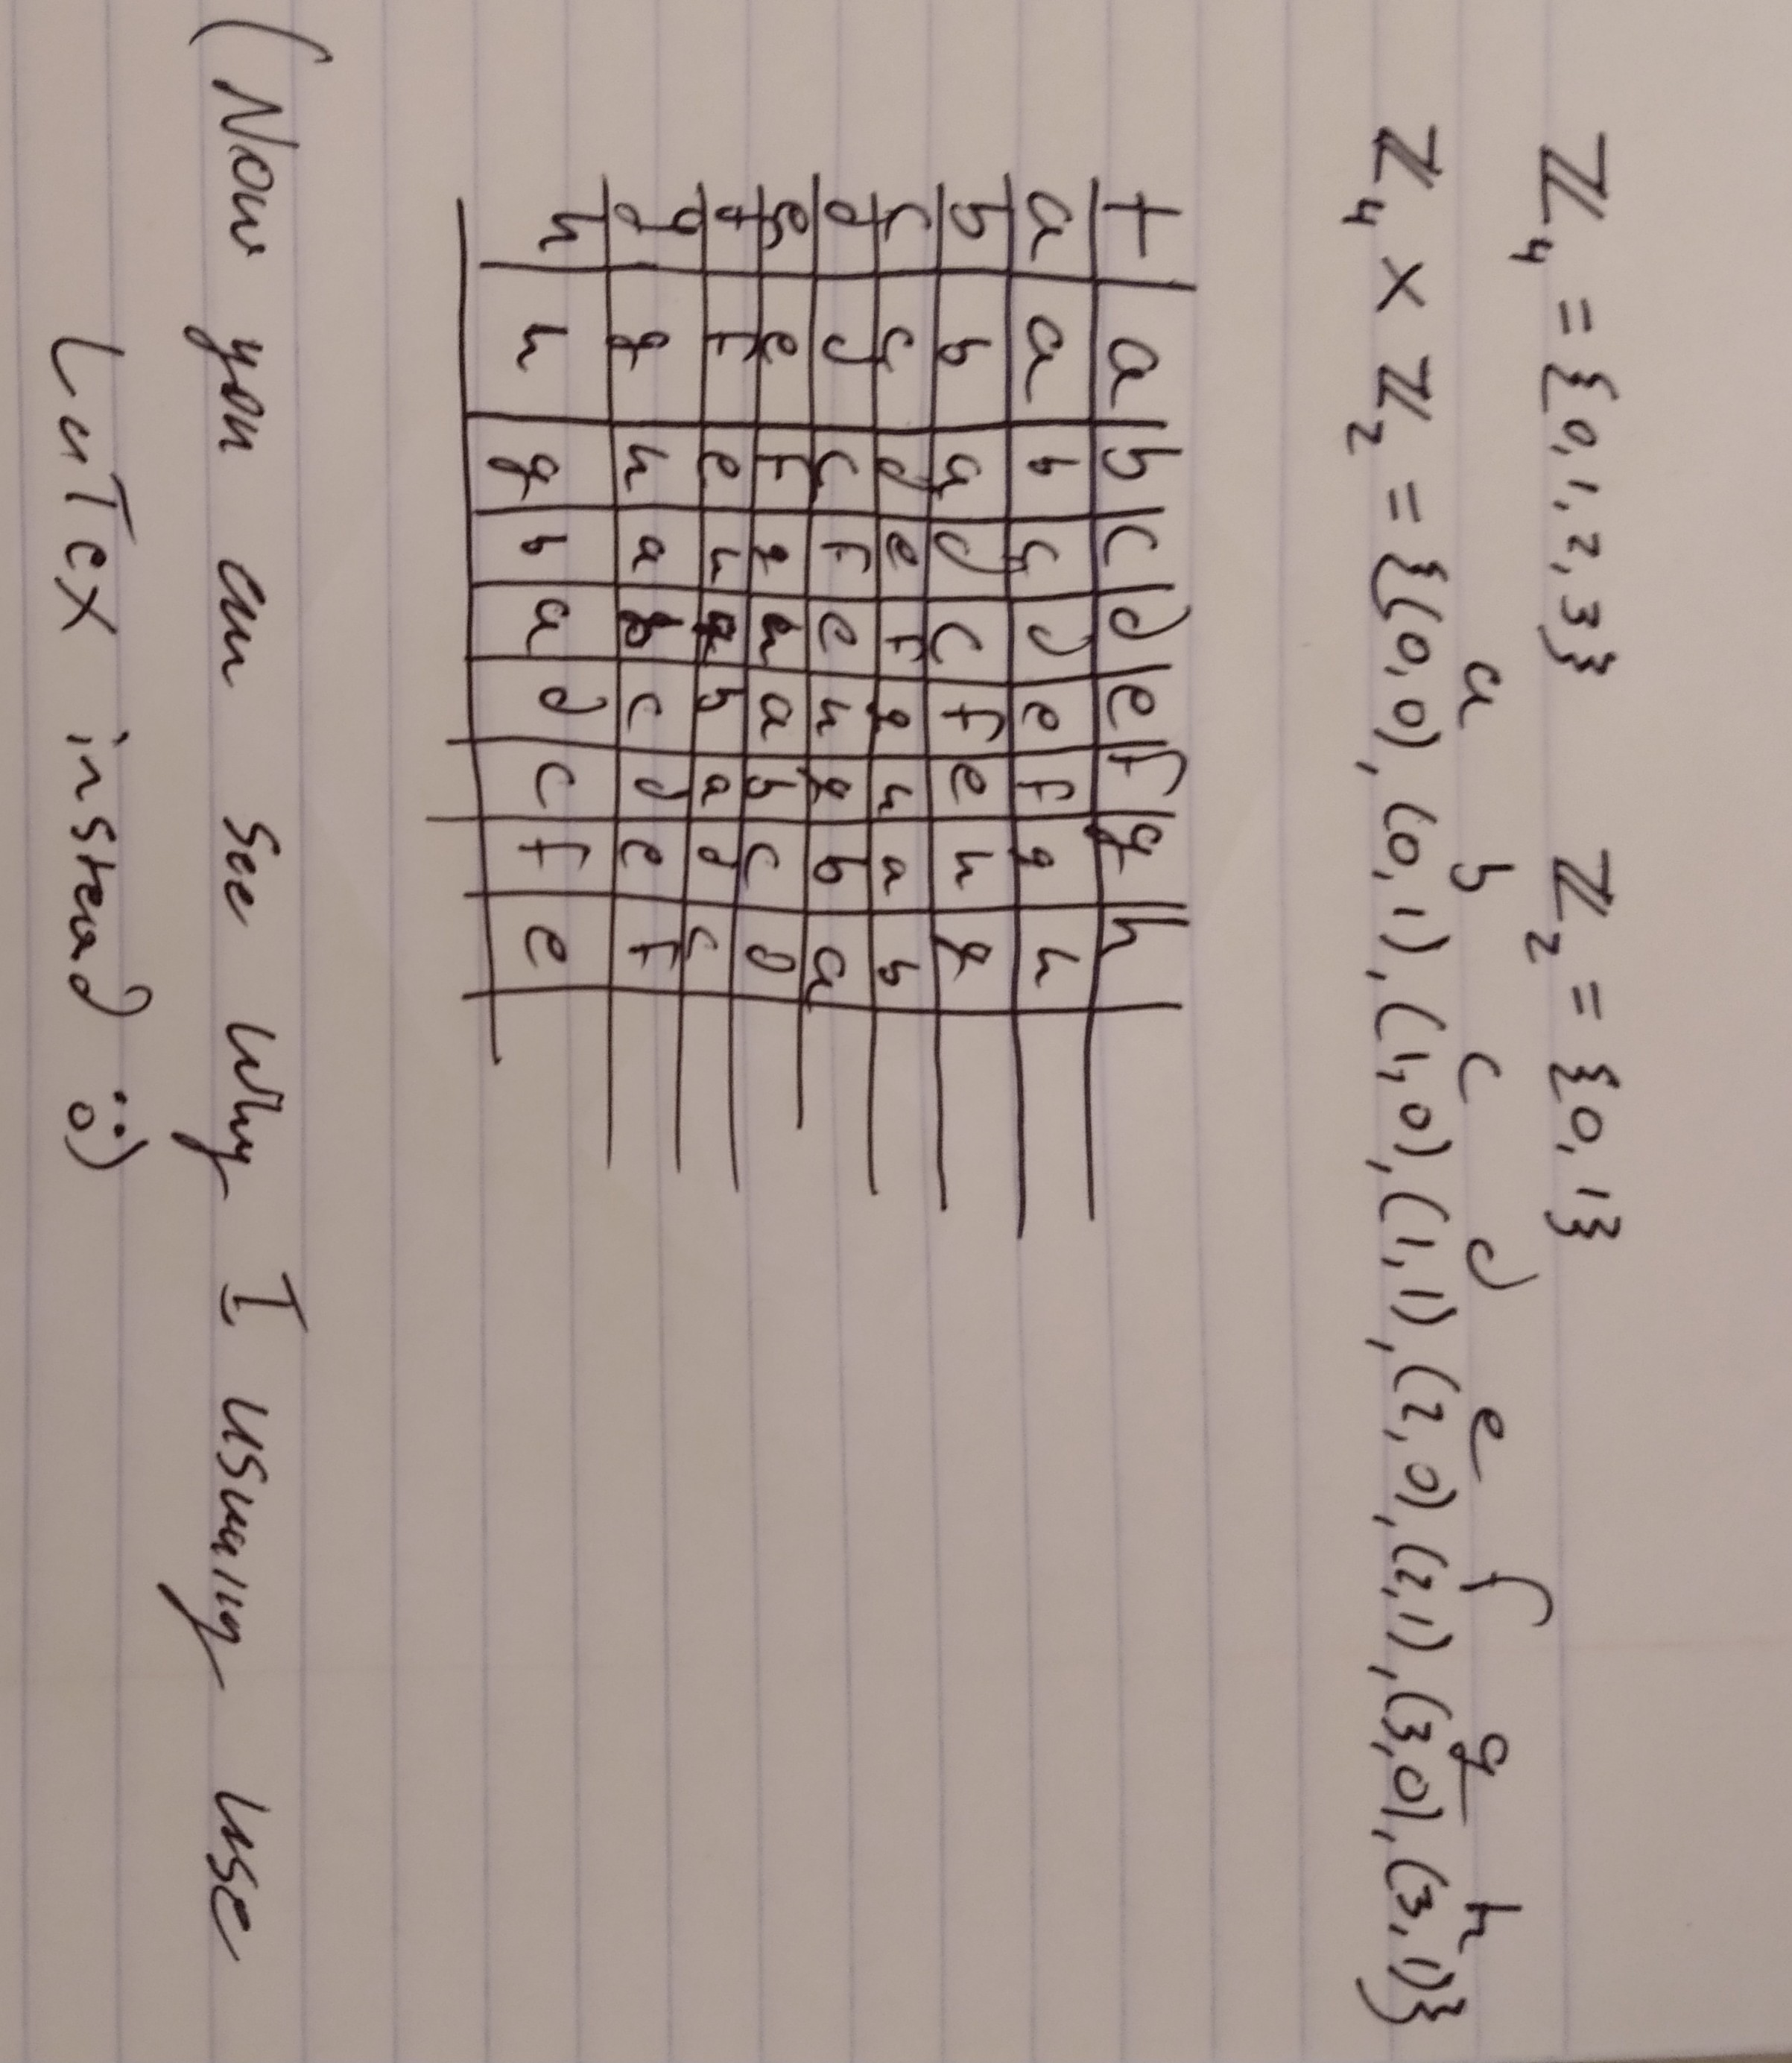
\includegraphics[angle =90]{z4xz2.jpg}}
\item Problem 5: Show that no proper subgroup of $S_4$ contains both $(1,2,3,4)$ and $(1,2)$.\begin{proof}\begin{remark}The group $S_n$ is generated by $(1,2,...,n)$ and $(1,2)$. \href{https://math.stackexchange.com/a/3703767}{\color{cyan}Proof.}\end{remark}Consider some subgroup $H\subseteq S_4$, such that $H\ni (1,2,3,4),(1,2)$. By our remark, any subgroup containing these two cycles must be exactly equal to $S_n$. Since both $(1,2,3,4),(1,2)\in H$, this proves that $H=S_4$ and thus $H\not\subset S_4$.
\end{proof}
\item Problem 10: Show that the following matrices form a subgroup of $GL_2(\C)$ isomorphic to $D_4$.\newline \qquad$\pm\begin{bmatrix}
1 & 0\\
0 & 1
\end{bmatrix}$,\qquad$\pm\begin{bmatrix}
i & 0\\
0 & -i
\end{bmatrix}$,\qquad$\pm\begin{bmatrix}
0 & 1\\
1 & 0
\end{bmatrix}$,\qquad$\pm\begin{bmatrix}
0 & i\\
-i & 0
\end{bmatrix}$.\begin{proof}We first check, for $G=\text{The matrices}$, $|G|=|D_4|=8$. This is true. Therefore there \emph{can} exist an isomorphism between the two. To show there must, $\forall a\in D_4$ we must find some $x\in G$ such that $|a|=|x|$. This will define the isomorphism $\phi:D_4\to G$.\begin{itemize}
    \item $\rho_{0}=e\in D_4$ has order 1. $\begin{bmatrix}
1 & 0\\
0 & 1
\end{bmatrix}\in G$ also has order 1.
    \item $\rho_{90}\in D_4$ has order 4. $\begin{bmatrix}
0 & -1\\
1 & 0
\end{bmatrix}\in G$ also has order 4.
    \item $\rho_{180}\in D_4$ has order 2. $\begin{bmatrix}
0 & 1\\
-1 & 0
\end{bmatrix}\in G$ also has order 2.
    \item $\rho_{270}\in D_4$ has order 4. $\begin{bmatrix}
0 & 1\\
-1 & 0
\end{bmatrix}\in G$ also has order 4.
    \item $\mu_1\in D_4$ has order 2. $\begin{bmatrix}
0 & 1\\
-1 & 0
\end{bmatrix}\in G$ also has order 2.
    \item $\mu_1\in D_4$ has order 2. $\begin{bmatrix}
-1 & 0\\
0 & 1
\end{bmatrix}\in G$ also has order 2.   
    \item $\mu_2\in D_4$ has order 2. $\begin{bmatrix}
0 & 1\\
1 & 0
\end{bmatrix}\in G$ also has order 2.    
    \item $\mu_3\in D_4$ has order 2. $\begin{bmatrix}
1 & 0\\
0 & -1
\end{bmatrix}\in G$ also has order 2.    
    \item $\mu_4\in D_4$ has order 2. $\begin{bmatrix}
0 & -1\\
-1 & 0
\end{bmatrix}\in G$ also has order 2.
\end{itemize}
Where $\rho_{\theta}$ defines a rotation by $\theta$ degrees, and $\mu_1$,$\mu_2$,$\mu_3$,$\mu_4$, define a flip vertically, horizontally, diagonally about $\overline{13}$, and diagonally about $\overline{24}$, respectively. Therefore, for every element of $D_4$, there exists exactly one element of $G$ with the same order, thus, $D_4\cong G$.
\end{proof}
\end{itemize}
\end{document}
